
\begin{figure}
\begin{tabular}{cc}
\subfigure[\label{fig:sub:explain}]{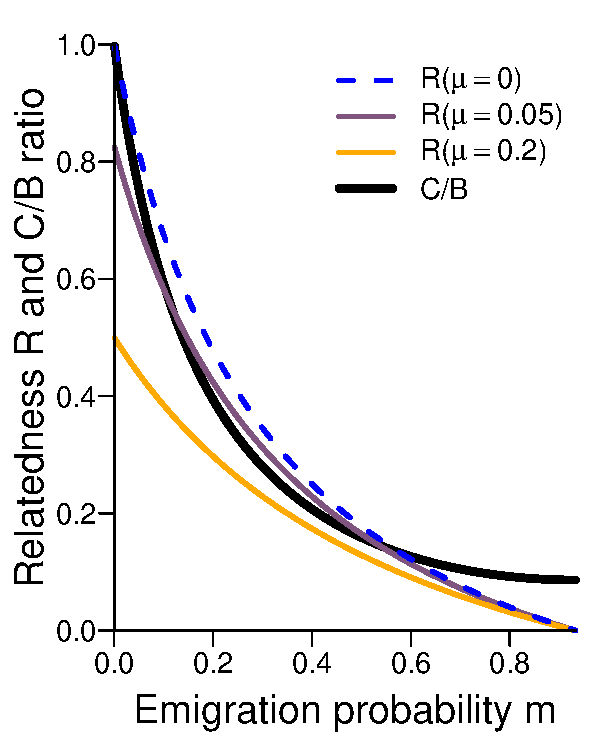
\includegraphics[width = \wpic]{../Programs/R/Pics/explainDB.pdf}}
&
\subfigure[\label{fig:sub:qualit}]{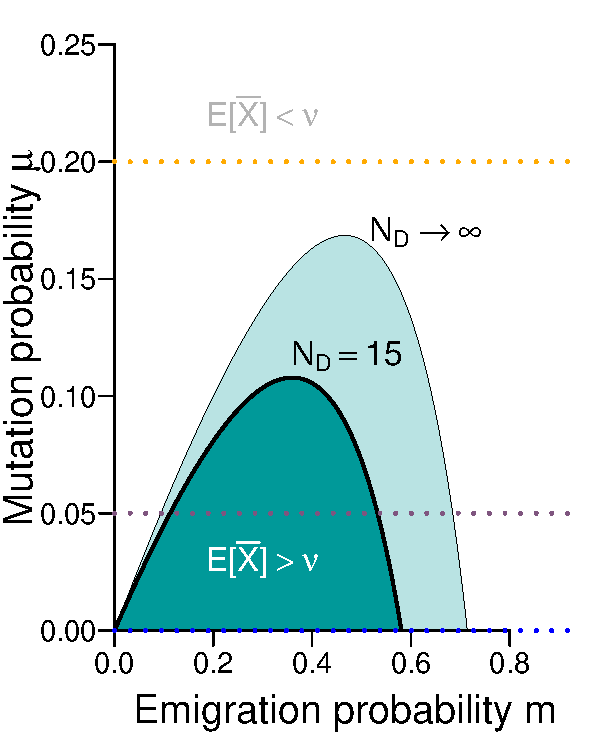
\includegraphics[width = \wpic]{../Programs/R/Pics/qualitDB.pdf}}
\end{tabular}
\caption{Understanding the effect of emigration $m$ on whether altruism is favored in the Death-Birth life-cycle. \subref{fig:sub:explain} Comparison of the $\mathcal{C}/\mathcal{B}$ ratio (thick black curve) and relatedness $R$ (thin curves) for different values of the mutation probability $\mu$ (same color code as previously). \subref{fig:sub:qualit} ($m$, $\mu$) combinations for which $\Esp{\overline{X}}>\mutbias$. The dotted horizontal lines correspond to the mutation values used in panel \subref{fig:sub:explain}. Unless specified, all other parameters are the same as in figure~\ref{fig:EX}.
}
\label{fig:DB}
\end{figure}
